\documentclass{beamer}
\usetheme{Warsaw}

\usepackage{polski}

\usepackage[utf8]{inputenc}
\usepackage[T1]{fontenc}

\usepackage{graphicx}
\usepackage{hyperref}

\usepackage{fancyvrb}

\usepackage{physics}

\setbeamertemplate{footline}[frame number]{}

\title{Optymalizacja półokreślona w wykrywaniu splątania kwantowego}
\author{Wojciech Wantka \\ promotor: dr inż. Piotr Mironowicz}
\date{}

\begin{document}

\frame{\titlepage}

\section{Cele}

\begin{frame}
    \begin{enumerate}
        \item Przegląd literatury odnośnie programowania półokreślonego.
        \item Wprowadzenie do metod informatyki kwantowej.
        \item Implementacja mechanizmu do wykrywania splątania kwantowego podanego stanu (z wykorzystaniem programowania półokreślonego).
        \item Sporządzenie dokumentacji.
    \end{enumerate}
\end{frame}

\section{Splątanie kwantowe -- wprowadzenie}

\subsection{Oznaczenia}

\begin{frame}
    \begin{itemize}
        \item $[n] \equiv \{0, 1, \ldots, n - 1\}$
        \item $\mathcal{H}$ -- przestrzeń Hilberta o wymiarze $n$ z ortonormalną bazą kanoniczną
            $$
                \mathcal{B} = \{\ket{i}\}_{i \in [n]}
            $$
        \item $\mathcal{H}_{AB} \equiv \mathcal{H}_{A} \otimes \mathcal{H}_{B}$
    \end{itemize}
\end{frame}

\subsection{Układy pojedyncze}

\begin{frame}
    \begin{exampleblock}{Stan czysty układu pojedynczego}
        W przestrzeni $\mathcal{H}$ stanem czystym nazywamy unormowany wektor

        $$
            \ket{\psi} = \sum \limits_{i \in [n]} \psi_{i} \ket{i}.
        $$
    \end{exampleblock}
\end{frame}

\begin{frame}
    \begin{exampleblock}{Stan mieszany układu pojedynczego}
        Jeżeli pojedynczy układ kwantowy z prawdopodobieństwem $p_{i}$ znajduje się w stanie czystym $\ket{\psi_{i}}$, to jego stan opisuje operator liniowy na $\mathcal{H}$, nazywany operatorem gęstości. Jest on postaci

        $$
            \rho \equiv \sum \limits_{i} p_{i} \ket{\psi_{i}} \bra{\psi_{i}}, 0 \leq p_{i} \leq 1, \sum \limits_{i} p_{i} = 1.
        $$
    \end{exampleblock}
\end{frame}

\begin{frame}
    \begin{exampleblock}{Ślad operatora}
        Jeżeli $\rho$ jest operatorem liniowym w przestrzeni z bazą ortonormalną $\ket{i}$, to ślad

        $$
            \textbf{Tr}[\rho] = \sum \limits_{i} \bra{i} \rho \ket{i}
        $$
    \end{exampleblock}
\end{frame}

\begin{frame}
    \begin{exampleblock}{Dodatnia określoność}
        Operator liniowy $\rho$ jest dodatnio określony, jeśli dla każdego $\ket{\psi}$ jest

        $$
            \bra{\psi} \psi \ket{\psi} \geq 0.
        $$

        Pisze się wtedy $\rho \geq 0$.
    \end{exampleblock}
\end{frame}

\begin{frame}
    \begin{alertblock}{Charakteryzacja operatorów gęstości}
        Operator $\rho$ działający na przestrzeni Hilberta $\mathcal{H}$ jest operatorem gęstości $\Leftrightarrow$

        \begin{enumerate}
            \item $\textbf{Tr}[\rho] = 1$
            \item $\rho$ jest operatorem dodatnio określonym
        \end{enumerate}
    \end{alertblock}
\end{frame}

\subsection{Układy złożone}

\begin{frame}
    \begin{alertblock}{}
        W przypadku układów złożonych można definiować pojęcie \textit{splątania} i \textit{separowalności} stanu kwantowego.
    \end{alertblock}
\end{frame}

\begin{frame}
    \begin{exampleblock}{Czysty stan układu złożonego}
        W przestrzeni $\mathcal{H}_{A} \otimes \mathcal{H}_{B}$ stanem czystym nazywamy unormowany wektor

        $$
            \ket{\psi} = \sum \limits_{i \in [n_{A}], j \in [n_{B}]} \psi_{ij} \ket{i_{A}} \ket{j_{B}}
        $$
    \end{exampleblock}
\end{frame}

\begin{frame}
    \begin{exampleblock}{Czysty stan splątany}
        Stan w przestrzeni $\mathcal{H}_{A} \otimes \mathcal{H}_{B}$, którego nie da się przedstawić w postaci

        $$
            \ket{\psi} = \ket{\psi_{A}} \ket{\psi_{B}}, \ket{\psi_{A}} \in \mathcal{H}_{A}, \ket{\psi_{B}} \in \mathcal{H}_{B},
        $$

        nazywamy stanem splątanym.
    \end{exampleblock}
\end{frame}

\begin{frame}
    \begin{alertblock}{Uwaga}
        Stan, który nie jest splątany, nazywamy stanem separowalnym.
    \end{alertblock}
\end{frame}

\begin{frame}
    \begin{exampleblock}{Czysty stan splątany -- Przykład}
        Przykładem stanu splątanego na $\mathbb{C} ^ {2} \otimes \mathbb{C} ^ {2}$ jest jeden ze stanów bazy Bella:

        $$
            \Phi ^ {+} = \frac{1}{\sqrt{2}} (\ket{00} + \ket{11})
        $$
    \end{exampleblock}
\end{frame}

\begin{frame}
    Niech

    $$
        \ket{\psi} = a \ket{0} + b \ket{1}
    $$

    $$
        \ket{\psi} = c \ket{0} + d \ket{1}
    $$

    Wtedy iloczyn tensorowy

    $$
        \ket{\psi} \ket{\phi} = ac \ket{00} + ad \ket{01} + bc \ket{10} + bd \ket{11}
    $$
\end{frame}

\begin{frame}
    Musiałoby być

    $$
        \begin{cases}
            ac = \frac{1}{\sqrt{2}} \\
            ad = 0 \\
            bc = 0 \\
            bd = \frac{1}{\sqrt{2}}
        \end{cases}
    $$

    Widać od razu, że warunki te są sprzeczne.
\end{frame}

\begin{frame}
    \begin{exampleblock}{Stan mieszany układu złożonego}
        W przypadku stanów mieszanych stan układu złożonego definiuje się jako operator gęstości $\rho^{AB}$ działający na przestrzeni $\mathcal{H}_{AB}$. Nazywa się go wtedy \textit{łącznym} operatorem gęstości. Definiujemy go ogólnie jako

        $$
            \rho ^ {AB} \equiv \sum \limits_{i, k \in [n_{A}]; j, l \in [n_{B}]} \rho_{ij, kl} ^ {AB} \ket{a_{i}} \bra{a_{k}} \otimes \ket{b_{j}} \bra{b_{l}},
        $$

        gdzie

        $$
            0 \leq \rho_{ij, kl} ^ {AB} \leq 1, \sum \limits_{i, k \in [n_{A}]; j, l \in [n_{B}]} \rho_{ij, kl} ^ {AB} = 1
        $$
    \end{exampleblock}
\end{frame}

\begin{frame}
    Definicja stanu separowalnego zostaje dla stanów mieszanych rozszerzona w stosunku do przypadku stanów czystych -- za taki stan uważa się nie tylko produkt dwóch stanów, ale każdą wypukłą kombinację produktów.
\end{frame}

\begin{frame}
    \begin{exampleblock}{Mieszany stan splątany}
        Jeżeli operator gęstości $\rho ^ {AB}$ działający na przestrzeni $\mathcal{H}_A \otimes \mathcal{H}_B$ da się zapisać w postaci

        $$
            \rho ^ {AB} = \sum \limits_{i} p_{i} \rho_{i}^{A} \otimes \rho_{i}^{B}, 0 \leq p_{i} \leq 1, \sum \limits_{i} p_{i} = 1,
        $$

        gdzie $\rho_{i}^{A}, \rho_{i}^{B}$ są operatorami gęstości działającymi na przestrzeni $\mathcal{H}_A, \mathcal{H}_B$ odpowiednio, to stan mieszany $\rho^{AB}$ nazywamy separowalnym.
    \end{exampleblock}
\end{frame}

\begin{frame}
    Okazuje się, że dla układów dwuczęściowych sprawa rozstrzygnięcia, czy operator gęstości działający na przestrzeni $\mathcal{H}_{AB}$ jest separowalny, jest problemem algorytmicznie NP-trudnym (zob. \cite{hor2009}). Dla przypadku $n_{A} = n_{N} = 2$ istnieje jednak bardzo ważne kryterium. Najpierw podamy jednak definicję tzw. \textit{częściowej transpozycji operatora gęstości}.
\end{frame}

\begin{frame}
    Niech $\mathcal{H}_{A} = \mathcal{H}_{B}$ są przestrzeniami Hilberta wymiaru $n$ z ortonormalnymi bazami $\ket{i}_{A}, \ket{j}_{B}$ odpowiednio. Niech $\rho$ jest operatorem gęstości na $\mathcal{H}_{AB}$ i niech w bazie $\ket{i_{A} j_{B}}$ jego reprezentacja macierzowa ma postać

    $$
        \begin{pmatrix}
            \rho_{00} & \rho_{01} & \cdots & \rho_{0, n - 1} \\
            \rho_{10} & \rho_{11} & \cdots & \rho_{1, n - 1} \\
            \vdots & \vdots & \vdots & \vdots \\
            \rho_{n - 1, 0} & \rho_{n - 1, 1} & \cdots & \rho_{n - 1, n - 1}
        \end{pmatrix}
    $$
\end{frame}

\begin{frame}
    \begin{exampleblock}{Częściowa transpozycja operatora gęstości}
        Częściową transpozycją operatora $\rho$ ze względu na podukład $\mathcal{H}_{B}$ nazywamy operator $\rho ^ {\Gamma}$, którego reprezentacja macierzowa w bazie $\ket{i_{A} j_{B}}$:

        $$
            \rho ^ {\Gamma} \equiv
            \begin{pmatrix}
                \rho_{00} ^ {T} & \rho_{01} ^ {T} & \cdots & \rho_{0, n - 1} ^ {T} \\
                \rho_{10} ^ {T} & \rho_{11} ^ {T} & \cdots & \rho_{1, n - 1} ^ {T} \\
                \vdots & \vdots & \vdots & \vdots \\
                \rho_{n - 1, 0} ^ {T} & \rho_{n - 1, 1} ^ {T} & \cdots & \rho_{n - 1, n - 1} ^ {T}
            \end{pmatrix}
        $$
    \end{exampleblock}
\end{frame}

\begin{frame}
    \begin{alertblock}{Częściowa transpozycja -- własności}
        Częściowa transpozycja ze względu na podukład $B$:

        \begin{enumerate}
            \item Zachowuje hermitowskość operatora
            \item Zachowuje ślad operatora
        \end{enumerate}
    \end{alertblock}
\end{frame}

\begin{frame}
    \begin{alertblock}{Kryterium Częściowej Transpozycji (\textit{Peres-Horodecki criterion}), zob. \cite{hor2009}}
        Operator gęstości $\rho$ działający w przestrzeni $\mathbb{C} ^ {2} \otimes \mathbb{C} ^ {2}$ jest stanem separowalnym $\Leftrightarrow$ operator $\rho ^ {\Gamma}$ jest operatorem gęstości.
    \end{alertblock}
\end{frame}

\section{Programowanie półokreślone}

\subsection{Definicje}

\begin{frame}
    \begin{exampleblock}{Dodatnia półokreśloność (positive semidefinity)}
        Macierz $S$ nazywa się \textit{dodatnio półokreśloną}, gdy dla każdego $v \in \mathbb{R} ^ {n}$ jest

        $$
            v ^ {T} S v \geq 0.
        $$

        Pisze się wtedy $S \geq 0$. Pisze się też $-S \leq 0$.
    \end{exampleblock}
\end{frame}

\begin{frame}
    \begin{exampleblock}{Problem programowania półokreślonego -- postać pierwotna}
        $$
            \begin{cases}
                \min \textbf{Tr}[CX] \\
                \text{ze względu na:} \\
                    \bullet \text{      } \textbf{Tr}[A_{i} X] = b_{i}, i=1, \ldots, p; \\
                    \bullet \text{      } X \geq 0,
            \end{cases}
        $$

        gdzie

        \begin{itemize}
            \item $X \in M_{n \times n}(\mathbb{R})$ jest macierzą symetryczną traktowaną jako zmienna;
            \item $C, A_{i} \in M_{n \times n}(\mathbb{R}), i = 1, \ldots, p$ są danymi macierzami symetrycznymi;
            \item $b_{i} \in \mathbb{R}, i = 1, \ldots, p$ są danymi liczbami.  
        \end{itemize}
    \end{exampleblock}
\end{frame}

\begin{frame}
    \begin{exampleblock}{Problem programowania półokreślonego -- postać dualna}
        $$
            \begin{cases}
                \min c ^ {T} x \\
                \text{ze względu na:} \\
                    \bullet \text{      } F(x) \leq 0 \\
                    \bullet \text{      } A x = b,
            \end{cases}
        $$

        gdzie

        $$
            F(x) = G + \sum \limits_{i = 1}^{m} x_{i} F_{i}
        $$

        dla

        $$
            x \in \mathbb{R} ^ m; c \in \mathbb{R} ^ {m}; G, F_{1}, \ldots, F_{m} \in \textbf{S} ^ {n}
        $$
    \end{exampleblock}
\end{frame}

\section{Narzędzia do SDP}

\subsection{Ogólnie}

\begin{frame}[fragile]
    \begin{enumerate}
        \item \verb+SDPA+ -- wiele interfejsów do różnych języków programowania; wersje wspierające zrównoleglanie obliczeń etc.
        \item \verb+YASS+ (C++)
        \item \verb+CSDP+ (C)
        \item \verb+DSDP+
    \end{enumerate}
\end{frame}

\subsection{Matlab}

\begin{frame}[fragile]
    \begin{enumerate}
        \item \verb+SeDuMi+
        \item \verb+SDPT3+
        \item \verb+YALMIP+
        \item \verb+CVX+
    \end{enumerate}
\end{frame}

\subsection{Python}

\begin{frame}[fragile]
    \begin{enumerate}
        \item \verb+cvxopt+ (Python [dostępne jako pakiet w PyPI central]) -- optymalizacja wypukła
    \end{enumerate}
\end{frame}

\subsection{Java}

\begin{frame}[fragile]
    \begin{enumerate}
        \item \verb+JOptimizer+ (Java, dostępne przez maven central)
    \end{enumerate}
\end{frame}

\subsection{R}

\begin{frame}[fragile]
    \begin{enumerate}
        \item \verb+sdpt3r+
        \item \verb+Rcsdp+ (interfejs do CSDP)
        \item \verb+Rdsdp+ (interfejs do DSPD)
    \end{enumerate}
\end{frame}

\section{JOptimizer}

\subsection{Przykład 1}

\begin{frame}
    $$
        \begin{cases}
            \min
                \Bigg(
                    \begin{bmatrix}
                        -\sqrt{\frac{21}{50}} & 0 \\
                        \frac{-\sqrt{2}}{5} & \frac{-1}{\sqrt{2}}
                    \end{bmatrix}
                    \begin{bmatrix}
                        x \\
                        y
                    \end{bmatrix}
                \Bigg) ^ {T}
                \Bigg(
                    \begin{bmatrix}
                        -\sqrt{\frac{21}{50}} & 0 \\
                        \frac{-\sqrt{2}}{5} & \frac{-1}{\sqrt{2}}
                    \end{bmatrix}
                    \begin{bmatrix}
                        x \\
                        y
                    \end{bmatrix}
                \Bigg)
            \\
            \Bigg(
                \begin{bmatrix}
                    1 & 0 \\
                    0 & 1
                \end{bmatrix}
                \begin{bmatrix}
                    x \\
                    y
                \end{bmatrix}
                +
                \begin{bmatrix}
                    2 \\
                    2
                \end{bmatrix}
            \Bigg) ^ {T}
            \Bigg(
                \begin{bmatrix}
                    1 & 0 \\
                    0 & 1
                \end{bmatrix}
                \begin{bmatrix}
                    x \\
                    y
                \end{bmatrix}
                +
                \begin{bmatrix}
                    2 \\
                    2
                \end{bmatrix}
            \Bigg)
            - 1.75 ^ {2} \leq 0
        \end{cases}
    $$
\end{frame}

\begin{frame}
    \begin{figure}
        \caption{Przykład 1 -- obszar dopuszczalny}
        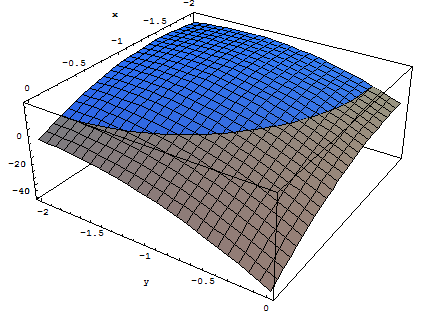
\includegraphics[scale=0.75]{images/example1_1.png}
    \end{figure}
\end{frame}

\begin{frame}
    \begin{figure}
        \caption{Przykład 1 -- obszar dopuszczalny}
        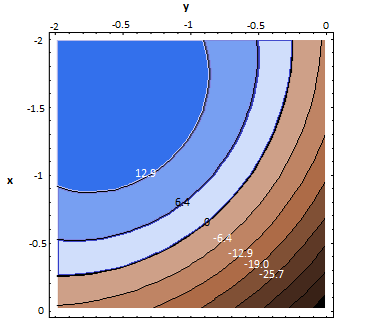
\includegraphics[scale=0.75]{images/example1_2.png}
    \end{figure}
\end{frame}

\begin{frame}[fragile]
    $$
        objectiveFunction(\textbf{x}) \equiv \textbf{q} \cdot \textbf{x} + r
    $$

    \begin{Verbatim}[fontsize=\small]
double[] q = {<q0>, <q1>, ..., <q_n>};
double r = <r_value>;
LinearMultivariateRealFunction objectiveFunction =
    new LinearMultivariateRealFunction(q, r);
    \end{Verbatim}
\end{frame}

\begin{frame}[fragile]
    \begin{Verbatim}[fontsize=\small]
private static double[] optimize(
    List<double[][]> fiMatrixList,
    double[][] gMatrix,
    OptimizationRequest optimizationRequest)
    throws JOptimizerException
{
    BarrierFunction barrierFunction =
        new SDPLogarithmicBarrier(fiMatrixList, gMatrix);
    BarrierMethod barrierMethod =
        new BarrierMethod(barrierFunction);
    barrierMethod.setOptimizationRequest(
        optimizationRequest);
    barrierMethod.optimize();

    return barrierMethod
        .getOptimizationResponse()
        .getSolution();
}
    \end{Verbatim}
\end{frame}

\section{Splątanie a SDP}

\begin{frame}
    \begin{exampleblock}{Świadek splątania}
        Obserwablę $W$ nazywa się \textit{świadkiem splątania}, gdy

        \begin{enumerate}
            \item $\textbf{Tr}[W \rho] \geq$ dla każdego separowalnego $\rho$
            \item $\textbf{Tr}[W \rho] < 0$ dla przynajmniej jednego splątanego $\rho$
        \end{enumerate}
    \end{exampleblock}
\end{frame}

\begin{frame}
    \begin{figure}
        \caption{Stany kwantowe jako wypukłe kombinacje}
        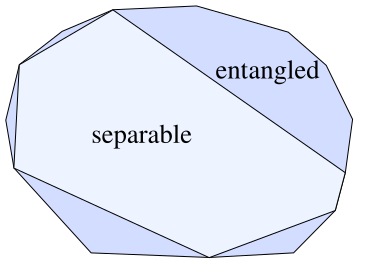
\includegraphics[scale=0.5]{images/convex-set.png}
    \end{figure}
\end{frame}

\section{Źródła}

\subsection{Splątanie kwantowe}

\begin{frame}
    \begin{thebibliography}{1cm}
        \setbeamertemplate{bibliography item}[article]
        \bibitem{dps2002}[1] A. C. Doherty, Pablo A. Parrilo, Federico M. Spedalieri, \textit{Distinguishing separable and entangled states} [arXiv:quant-ph/0112007].
        \bibitem{dps2003}[2] A. C. Doherty, Pablo A. Parrilo, Federico M. Spedalieri, \textit{A complete family of separability criteria} [arXiv:quant-ph/0308032].
        \bibitem{hor2009}[3] R. Horodecki, P. Horodecki, M. Horodecki, K. Horodecki, \textit{Quantum entanglement}, Revievs of Modern Physics \textbf{81}, 865 (2009) [arXiv:quant-ph/0702225].
    \end{thebibliography}
\end{frame}

\subsection{Programowanie półokreślone}

\begin{frame}
    \begin{thebibliography}{1cm}
        \setbeamertemplate{bibliography item}[book]
        \bibitem{} Stephen Boyd, Lieven Vandenberghe, \textit{Convex Optimization} [\url{https://web.stanford.edu/~boyd/cvxbook/}].
        \setbeamertemplate{bibliography item}[online]
        \bibitem{helmberg} \url{www-user.tu-chemnitz.de/~helmberg/semidef.html}.
    \end{thebibliography}
\end{frame}

\subsection{Optymalizacja -- ogólnie}

\begin{frame}
    \begin{thebibliography}{1cm}
        \setbeamertemplate{bibliography item}[online]
        \bibitem{} \url{https://en.wikipedia.org/wiki/List_of_optimization_software}.
        \setbeamertemplate{bibliography item}[article]
        \bibitem{} Ehsan Elhamifar, Guillermo Sapiro, Allen Yang, S. Shankar Sastry, \textit{A Convex Optimization Framework for Active Learning}.
    \end{thebibliography}
\end{frame}

\end{document}
